\documentclass[tikz,border=3mm]{standalone}
\usepackage{tikz}
\usetikzlibrary{arrows.meta,positioning,shapes.geometric,fit,backgrounds,calc}

\begin{document}
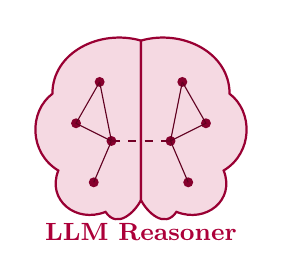
\begin{tikzpicture}

% Define a nice brain icon macro/scope
\def\drawbrain#1#2{
  \begin{scope}[shift={(#1)}, scale=#2]
    % Outer silhouette of brain (two hemispheres / lobes)
    % Left hemisphere
    \draw[fill=purple!15, draw=purple!80!black, line width=0.8pt]
      (0, 0.75) 
      .. controls (-0.35, 0.85) and (-0.75, 0.65) .. (-0.75, 0.3)
      .. controls (-0.95, 0.15) and (-0.95, -0.2) .. (-0.7, -0.35)
      .. controls (-0.8, -0.6) and (-0.55, -0.8) .. (-0.3, -0.7)
      .. controls (-0.2, -0.85) and (-0.05, -0.7) .. (0, -0.6)
      -- cycle;

    % Right hemisphere
    \draw[fill=purple!15, draw=purple!80!black, line width=0.8pt]
      (0, 0.75) 
      .. controls (0.35, 0.85) and (0.75, 0.65) .. (0.75, 0.3)
      .. controls (0.95, 0.15) and (0.95, -0.2) .. (0.7, -0.35)
      .. controls (0.8, -0.6) and (0.55, -0.8) .. (0.3, -0.7)
      .. controls (0.2, -0.85) and (0.05, -0.7) .. (0, -0.6)
      -- cycle;

    % Central fissure
    \draw[purple!80!black, line width=0.9pt] (0, 0.72) -- (0, -0.58);

    % Neural network nodes and synaptic connections inside left lobe
    \fill[purple!70!black] (-0.35, 0.4) circle (1.2pt);
    \fill[purple!70!black] (-0.55, 0.05) circle (1.2pt);
    \fill[purple!70!black] (-0.25, -0.1) circle (1.2pt);
    \fill[purple!70!black] (-0.4, -0.45) circle (1.2pt);
    \draw[purple!50!black, line width=0.4pt] (-0.35, 0.4) -- (-0.55, 0.05) -- (-0.25, -0.1) -- (-0.4, -0.45);
    \draw[purple!50!black, line width=0.4pt] (-0.35, 0.4) -- (-0.25, -0.1);

    % Neural network nodes and synaptic connections inside right lobe
    \fill[purple!70!black] (0.35, 0.4) circle (1.2pt);
    \fill[purple!70!black] (0.55, 0.05) circle (1.2pt);
    \fill[purple!70!black] (0.25, -0.1) circle (1.2pt);
    \fill[purple!70!black] (0.4, -0.45) circle (1.2pt);
    \draw[purple!50!black, line width=0.4pt] (0.35, 0.4) -- (0.55, 0.05) -- (0.25, -0.1) -- (0.4, -0.45);
    \draw[purple!50!black, line width=0.4pt] (0.35, 0.4) -- (0.25, -0.1);

    % Cross-hemisphere connection
    \draw[purple!60!black, line width=0.4pt, dashed] (-0.25, -0.1) -- (0.25, -0.1);
  \end{scope}
}

\drawbrain{0,0}{1.5};
\node[font=\bfseries\small, text=purple!90!black] at (0, -1.3) {LLM Reasoner};

\end{tikzpicture}
\end{document}
